\section{The Symmetry Breaking Problem}
\label{cap:2}

Formally, a symmetry system can be defined as a system in which the processes are in an equivalence relation, this means that if the processes run the same code, it is possible to permute the nodes without changing the behaviour of the system. One example of this state would be a ring in which there is no unique identifier for every node. If we consider a message passing system in which the initial state of symmetry between all processes, it is possible to find a synchronous execution in which the processes will continue in the same initial state. In this case, it is necessary a mechanism to break the symmetry, in the contrary, the system cannot escape from the initial state.
%as shown in \cite{angluin1980local} by Angluin.

Symmetry breaking is one of the most extensively studied problems in distributed computing. The fundamental problems on graph include the maximal matching, vertex colouring, ruling sets and \textit{MIS}. The last one can be considered as the central problem because all the others can be reduced to it, as shown in  \cite{}.

In the next section, a formal definition of the maximal independent set is given and a discussion on the sequential algorithm vs distributed algorithm is presented. Besides that, a theoretical analysis on time and message complexity is described.     

\subsection{Maximal Independent Set}

\theoremstyle{definition}
\begin{definition}

Given a undirected graph $G = (V,E)$, a set of vertices $S \subseteq V$ is called a Maximal Independent Set \textbf{MIS} if it satisfied the following properties:   

\begin{enumerate}
  \item the set S in an independent set meaning that no two vertices $v,u \in S$ are adjacent,
  \item the set S is maximal, with regards to independence, meaning that for each node $v \notin S$, there 
    exist a neighbour u of v such that $u \in S$.
\end{enumerate}

\end{definition}

Figure \ref{fig:graph1} show an example of undirected graph with 8 nodes and 14 edges. The goal if to find a set of nodes in which every node is part of the set or it is neighbour of some node that is part of the set. It is possible to find more that one solution to the same instance as shown in the figure \ref{fig:mis1}  
 
\begin{figure}[h]
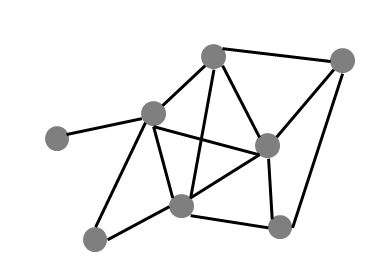
\includegraphics[width=0.4 \linewidth, height=3cm]{c2-graph.PNG} 
\caption{General graph G}
\label{fig:graph1}
\end{figure}
 
\begin{figure}[h]
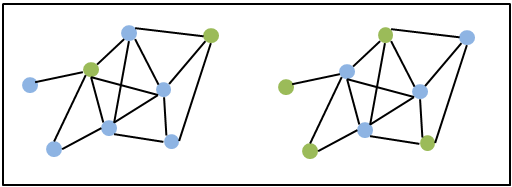
\includegraphics[width=0.4 \linewidth, height=3cm]{c2-graph-mis1.PNG}
\caption{Solution 1 for MIS of G}
\label{fig:mis1}
\end{figure}

The algorithm \ref{algorithm:secuential-mis} describe a general sequential algorithm to find the maximal independent set of a general graph. The time complexity is $O(N)$ since in the worst case, the algorithm has to check every node. Another approach to improve this time is desirable. In the next section, two distributed approach to solve the \textit{MIS} problem are presented.

\begin{algorithm}
 \caption{Sequential Maximal Independent Set}
 \label{algorithm:secuential-mis} 

\SetAlgoLined
\KwResult{IS Set of nodes}
\KwData{ $G(V,E)$ Graph}
    \While {V is not empty}{
        Choose a node $v \in V$
            Add v to the set IS\;
            Remove from V the node v and all its neighbours\;
        }
    
 
\end{algorithm}
 

 
\subsection{Distributed Maximal Independent Set}

A logarithmic lower bound is always desirable and the difficulty to find it in sequential algorithms to the \textit{MIS} problem motivate the development of distributed algorithm. In 1986, the first distributed algorithm was proposed independently by Luby \cite{luby1986simple} and Alon \textit{et al.} \cite{alon1986fast}. Both algorithms are randomised and have $O(log N)$ lower bound. Until now, there are faster than the best distributed deterministic algorithms for general graphs. There have been some improvements for special cases, for instance \cite{panconesi1996complexity} propose a $O(\delta + log^* N)$ algorithm, however  the originals algorithm are still faster when $\delta = \omega(log N)$ and if the running time is expressed solely as a function of $N$. It is worth to mention that all algorithms exposed forward are in the synchronous model. 

The algorithm\ref{algorithm:luby-mis} describe the original Luby's algorithm. TO BE COMPLETED ........


\begin{algorithm}
 \caption{Luby's Algorithm, code for each node i = 1 to N}
 \label{algorithm:luby-mis} 

\SetAlgoLined
\KwResult{MIS Maximal Independent Set}
\KwData{ $G(V,E)$ Graph}
    \While {V is not empty}{
        Choose a random set of vertices $S ⊆ V$, by selecting each vertex $v$ independently with probability $1/(2d(v))$, where d is the degree of $v$\;
        For every edge in E, if both its endpoints are in the random set S, then remove from S the endpoint whose degree is lower. Break ties arbitrarily, e.g. using a lexicographic order on the vertex names\;
        Add the set S to IS\;
        Remove from V the set S and all the neighbours of nodes in S\;
        }
\end{algorithm} 





\theoremstyle{theorem}
\begin{theorem}

Algorithm \ref{algorithm:luby-mis} computes a maximal independent set for any graph  in O(log n) rounds with high probability.

\end{theorem}


The algorithm \ref{algorithm:main-mis} was proposed in \cite{yves2009optimal} and it is the one used for the simulations in this project. The correctness of the algorithm it is very intuitive. This algorithm operates in synchronous rounds. In line 2, every process select a random number to in order to break the symmetry with its neighbours, line 3 makes sure that if a vertex v join the MIS, no other neighbour of v join the MIS at the same time, this is true because the execution  occurs in rounds. the line 4 makes sure that any vertex that has a neighbour in the MIS, join the MIS at any point. 

\begin{algorithm}
 \caption{MIS Algorithm, code for each node from i = 1 to N}
 \label{algorithm:main-mis} 

\SetAlgoLined
\KwResult{MIS Maximal Independent Set}
\KwData{ $G(V,E)$ Graph}
    \While {V is not empty}{
        Selects a random number $r(v)$ between [0,1] and sends to its neighbours\;
        If $r(v) < r(w)$ for all neighbours $w \in N(v)$ numbers, remove myself from V and enter to the MIS \newline
        Inform my neighbours that I am a MIS member and terminate\;
        If I heard that my neighbour is MIS, remove myself from the V and terminate\;
        }
\end{algorithm}

\newpage